\documentclass[12pt]{article}



\usepackage{hyperref}

\usepackage{listings}
\usepackage[margin=1.25in]{geometry}
\usepackage{graphicx}
\graphicspath{ {./images/} }
\usepackage{imakeidx}
\makeindex[columns=3, title=Alphabetical Index, intoc]

\begin{document}

\begin{titlepage}

\title{%
  HW1: Mid-term assignment report\\
  \large  Testing and Software Quality\\}

\author{Rafael Remígio 102435}

\maketitle

\vfill
\begin{center}

	Departamento de Electrónica, Telecomunicações e Informática\\
       Universidade de Aveiro\\ Year 2022/2023
\end{center}



\end{titlepage}

\tableofcontents


\section{Introduction}

\subsection{Overview of the work} 

In this assignment the web application developed provides real-time information parameters related to the air quality of a certain location.

\subsection{Current limitations} 


\section{Product specification}


\subsection{Functional scope and supported interactions }


\subsubsection{Actors}

Possible Actors of the proposed product:

\begin{itemize}

\item Individuals - People who want to check the air quality in their immediate surroundings, such as their home, office, or neighborhood.

\item Public Health Officials - Officials who want to monitor air quality in a particular region or city to make informed decisions on public health policies.

\end{itemize}


\subsubsection{Use Cases}
The WebApp provides two use cases:

\begin{enumerate}

\item  Real-time Air Quality Monitoring. Provides real-time air quality levels in a particular location. This information consists of the specific parameters: 
	\begin{itemize}
		\item Particulate Matter PM2.5
		\item Particulate Matter PM10
		\item Carbon Monoxide CO
		\item Nitrogen Dioxide NO2
	\end{itemize}
	
\item access and view statistics of the cache's usage:
	\begin{itemize}
		\item Misses
		\item Hits
		\item Acesses
	\end{itemize}

\end{enumerate}


\subsection{System architecture}

\subsubsection{Architecture}
The application's Architecture is very basic and allows for easy maintenance and API evolution. The Controller handles communication between the WebApp and the backend. The Service Layer is composed of two distinct services. The Weather Service (responsible for providing the Air Quality for a certain region) utilizes a Geocoding API in order to transform an address or location string into coordinates. It communicates with two different Air Quality API's. In order to provide more constant availability and resilience, one acts as a backup when the main API is down. These API's provide Air Quality data for a certain location based on latitude and longitude.
In order to reduce query times, a caching system using a key-value database was also introduced. The objects cached have a specific Time to Live that is easily configurable.
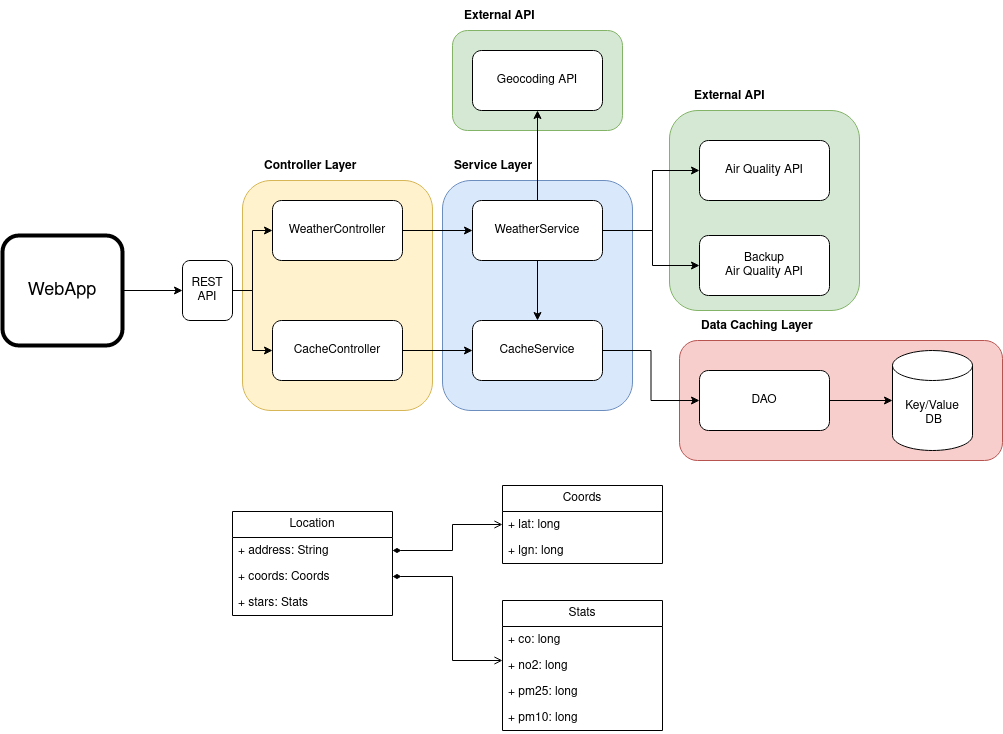
\includegraphics[scale=.4]{architecture.png}

\subsubsection{Technologies and API's Used}

The very basic User Interface was constructed using ReactJS. It interacts with the Backedn througth a RestAPI. The backend was built using Spring Boot. For an in memory database I used Redis. The Geolocation Api chosen was Open Cage. The primary Air Quality API is the OpenWeather API. The backup Air Quality API is the OpenMeteo API.

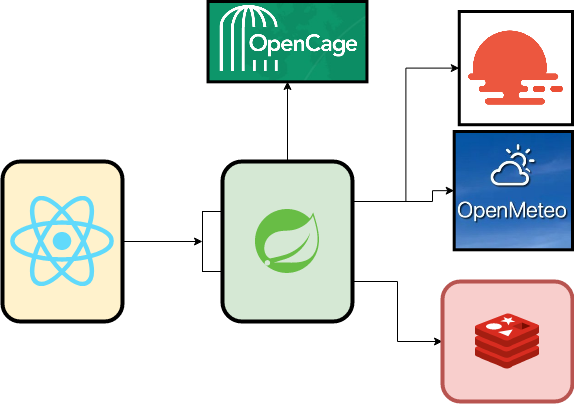
\includegraphics[scale=.4]{TechFrameworks.png}



\subsection{API}

The API has two endpoints:

\begin{enumerate}
	
	\item \textbf{GET} /weather?local=\textit{\{local\}} \\
	Query Params: 
	\begin{itemize}
			\item \textbf{Required} - local: Address, Country or City .
	\end{itemize}
		
	
	Response Body: \\ 
	\begin{lstlisting}
	{
	 "coords":{
	 	"lat":40.7275536,
	 	"lgn":-8.5209649
	 	},
	 "stats":{
	 	"co":150.0,
	 	"no2":6.5,
	 	"pm25":9.4,
	 	"pm10":11.5
	 	},
	 "location":"aveiro"
	}
	\end{lstlisting}
	
	
	\item \textbf{GET} /cacheInfo\\
	Response Body: \\
	\begin{lstlisting}
		{
		"hits":5,
		"misses":10,
		"acesses":15
		}
		
	\end{lstlisting}

\end{enumerate}

\section{Quality assurance}

\subsection{Logging}

Logging is a crucial aspect of software development that plays a vital role in supporting production and debugging activities. \\
Logging was conducted using the slf4j Logger class has it provides an easy integration with the Spring Boot Application.\\
Each log message contains a timestamp, method invocation details, custom log messages, and other contextual data. Additionally, each log entry is assigned a logging level identifier, providing a way to categorize and prioritize log entries based on their significance.\\
I followed logging principles and best practices - such as: logging at the correct evel, providing meaningfull messages, etc - in order to provide meaningfull logs.

\subsection{Overall strategy for testing}


\subsection{Unit and integration testing}

implemented and 

\subsection{Functional testing}

\subsection{Code quality analysis}

For static sode analysis I used throughout the entirety of the project the SonarQube platform. It helped me identify potential bugs and vulnerabilities, improve code my code quality, and find code smells and possible anti-patterns. In conjunction with with static code anylisis I also used the SonarQube platform in order to evaluate the code coverage of tests implemented.

\includegraphics[scale=0.35]{sonarQube.png}

\subsection{Continuous integration pipeline}

\section{References \& resources}

GitRepository can be found at \"my github\".

\subsection{Reference materials}

\end{document}